\documentclass{article}

% if you need to pass options to natbib, use, e.g.:
%     \PassOptionsToPackage{numbers, compress}{natbib}
% before loading neurips_2024

% ready for submission
\usepackage[final]{neurips_2024}

% to compile a preprint version, eg, for submission to arXiv, add add the
% [preprint] option:
%     \usepackage[preprint]{neurips_2024}

% to compile a camera-ready version, add the [final] option, e.g.:
%     \usepackage[final]{neurips_2024}

% to avoid loading the natbib package, add option nonatbib:
%    \usepackage[nonatbib]{neurips_2024}

\usepackage[utf8]{inputenc} % allow utf-8 input
\usepackage[T1]{fontenc}    % use 8-bit T1 fonts
\usepackage{hyperref}       % hyperlinks
\usepackage{url}            % simple URL typesetting
\usepackage{booktabs}       % professional-quality tables
\usepackage{amsfonts}       % blackboard math symbols
\usepackage{nicefrac}       % compact symbols for 1/2, etc.
\usepackage{microtype}      % microtypography
\usepackage{xcolor}         % colors
\usepackage{authblk}
\usepackage{graphicx}
\usepackage{placeins}

%------------------------------------------------------------------------------
% Final Project: Predicting Urban Micro-Climates
%------------------------------------------------------------------------------
\title{Predicting Micro-Climates: Time-Series Approach to Hourly Temperature and Humidity Forecasting \\ 
\large CS 439 - Final Project Report}

\author{%
      \begin{center}
        {\large May 10, 2026} \\
        {\large Anna Lu (al1678)} \\
        {\large Artem Ivaniuk (ai392)} \\
        {\large Christopher DSouza (cd1001)} \\
        \vspace{0.5cm}
    \end{center}
}

\begin{document}

\maketitle

%------------------------------------------------------------------------------
% 1. Title and Team Information (already included above)
%------------------------------------------------------------------------------
\section{Abstract}
%------------------------------------------------------------------------------
% 2. Research Question and Motivation
%------------------------------------------------------------------------------
\subsection{Research Question and Motivation}

Research Question: To what extent can a multivariate time-series model accurately forecast micro-climate conditions, specifically hourly temperature, using publicly available meteorological data?

Motivation: 
As opposed to macroenvironments that are well-described by their general pattern, local areas exhibit distinct temperature changes, climate factors, humidity perseverance, and can be much more interesting for modeling due to each individual location's combination of factors -- going even as far as building density, vegetation, and topography. These minute changes from area to area can be linked to the downflow effects on energy consumption, public health, air quality, collective decisions in urban planning, and more. 


Our dive into this research question is motivated by two main factors. First, as Math, Econ, and CS majors, we are highly interested in learning to apply the data science skills we learn in this class to data that breaks the `independence' assumption between nearby variables and lean into the world of time-series forecasting. Second, accurate microclimate predictions would have serious implications on the individual decisions in housing decisions, health upkeep, and green energy concerns. In the ideal situation, we would want our project to be an MVP for empowering local officials to know their microclimates in better detail and be able to issue more accurate climate-oriented decisions. 

\subsection{GitHub Repository And Video}
Here is our GitHub repository for the project: \url{https://github.com/MazaArt/time_series_micro_climates} and it is structured as follows:

\begin{itemize}
    \item \texttt{example\_env.txt}, an example file for the .env, which is necessary to store the NOAA API token 
    \item \texttt{data/}, which stores both raw and processed datasets
    \begin{itemize}
        \item \texttt{raw/}, downloaded files such as the list of stations we are using, hourly meteorology data, and precipitation data (we did not end up using precipitation data)
        \item \texttt{processed/}, merged datasets used for modeling, mainly \texttt{minimum\_hourly\_merged.csv}
    \end{itemize}
    \item \texttt{src/}, which contains the project notebooks
    \begin{itemize}
        \item \texttt{data\_pull.ipynb}, used for downloading and cleaning NOAA data
        \item \texttt{rudimentary\_forecast.ipynb}, an implementation of naive 'report last seen value' and linear regression methods
        \item \texttt{time\_series\_forecast.ipynb}, the main time series decomposition and SARIMA modeling notebook
    \end{itemize}
    \item \texttt{proposal/}, which stores proposal drafts and planning material
    \item \texttt{final\_report/figures\_forecast/}, where we saved the figures from the forecasting notebooks to use in this report
\end{itemize}

Link for the video: \url{https://rutgers.zoom.us/rec/share/nm1GisdgoonxlwpKZYMF2CEAUFe8reT-saAgg5_1Xx82UQwEElPODMXWxGrm5BlN.j-NduhxV9vVfIaXP}

Passcode: s4L=QE0C
%------------------------------------------------------------------------------
% 3. Data Sources
%------------------------------------------------------------------------------
\section{Data Source and Cleaning}

The data pull notebook collects information from NOAA National Climatic Data Center (\url{"https://www.ncei.noaa.gov/data/global-hourly/access"}) from the start of 2020 through the start of 2026 (the actual data present does not run until this time spot, see below) for the three hard-coded station IDs corresponding to LaGuardia, JFK, and Newark Liberty. For each station and calendar year overlapping that range, the notebook downloads CSV exports from NOAA NCEI global hourly URLs. Each file is identified by station and year, then read with pandas and trimmed down to UTC timestamps that fall within the configured window.

Respectively, we are pulling the following data from the NOAA:
\begin{itemize}
    \item Local Climatological Data (LCD): hourly observations of temperature, humidity, dew point, wind speed, wind direction, pressure, and sky conditions. 
    \item Hourly Precipitation Data (HPD): we aimed to incorporate the impact of rainfall on temperature and humidity, so we pulled the HPD data for the stations above.
\end{itemize}

The downloaded rows contain LCD-style coded weather fields such as temperature and dew point values stored in tenths. Helper functions split out the numeric portion, remove missing or sentinel values like 9999 (NOAA's default for missing values), and convert everything into a long-format table with columns for station, timestamp, datatype, and value so that we are able to use this data easily in the future. We then saved both outputs into separate CSV files under \texttt{data/raw/} so we could rerun later stages without repeatedly pulling data from NOAA.

During cleaning, we pivoted the long tables into wide hourly tables indexed by station and observation time. If duplicate keys appeared, we averaged them. We also prefixed column names so precipitation and meteorology variables would not collide (we later chose not to use precipitation data at all, but this was unknown at the stage of data pull). The two wide tables were merged with an outer join on station and UTC timestamp to preserve all observations from either source. After sorting the merged dataset, we added Eastern local time using \texttt{America/New\_York} along with helper columns for local hour and month that we later used in the hourly plots. The final merged dataset was saved as \texttt{data/processed/minimum\_hourly\_merged.csv}. At this stage, the main issue was that the data did not map perfectly onto an hourly grid, since the NOAA archive reports observations at whatever times stations actually logged them. Because of that, later forecasting steps still needed resampling and alignment. For most of our uses, we just chose to average out all the points in the hour and call that the hourly figure.

For the testing set, we planned to reserve all of calendar year 2025 as a holdout period. The idea was to train on all observations before January 1, 2025 and evaluate forecasts across every hour of 2025. However, the Newark dataset we focused on stopped in late summer 2025 (specifically on August 25th) rather than continuing through December. After checking the pipeline, we found this was not caused by the merge or cleaning code. The later 2025 rows simply were not present in the NOAA global-hourly files when we pulled the dataset. The forecast notebook still specifies a test window extending into 2026, but pandas automatically intersects that with the timestamps that actually exist. As a result, the reported forecast errors only cover the months available in the dataset. Once NOAA backfills the remaining months, we will be able to rerun the code to get the full year of forecast errors, but the current plots only go until August 25th of 2025 so far.

\section{Rudimentary Forecasting}

To ensure that we have an idea of how good our forecasting model is in the next step we included an intermediate phase in \texttt{rudimentary\_forecast.ipynb}, where we tested out with 2 different models. One being the "Naive" approach where we simply try predicting the temperature in the next hour will be the same as the current hour - also known as the "Last Observed Value" model. And for comparison, we also incorporated a simple linear regression model. To make this work with time-based data, we performed feature engineering by converting the local hour into cyclical $sin$ and $cos$ components. This was done to help the model recognize that hour 23 and hour 0 are close together, rather than treating time as a purely linear feature. Establishing these baselines for more complex time series forecasting was crucial because as it proved that standard regression isn't enough for this kind of data. The linear model's high MSE of $18.26$ once again highlights the need for the autoregressive components which we included in our final SARIMAX model.

\FloatBarrier
\begin{figure}[htbp]
  \centering
  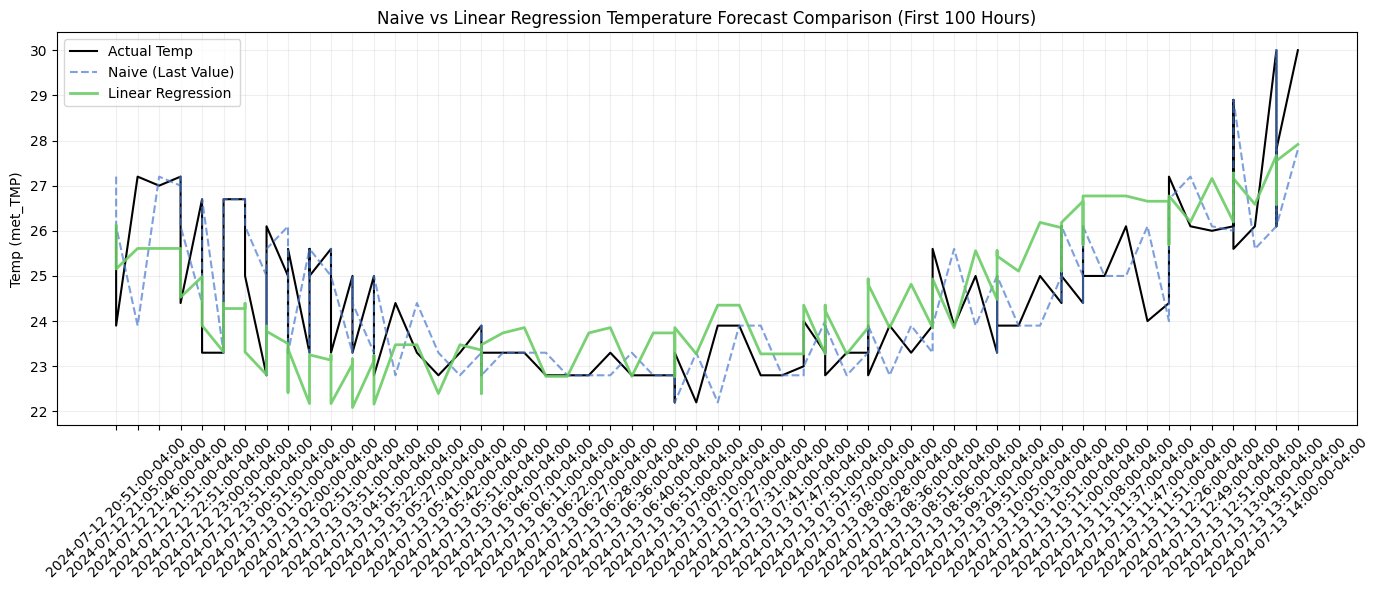
\includegraphics[width=\linewidth]{figures_forecast/naive_linRegr.png}
  \caption{Naive vs Linear Regression Comparison}
  \label{fig:naive_vs_linear}
\end{figure}
\FloatBarrier

As we can tell from Figure \ref{fig:naive_vs_linear} that surprisingly a simple naive approach perform much better than a linear regression model. Normally we will assume that a linear regression model will perform better but due to the fact that the time between each interval, in this case each hour, is so short a cyclical model without memory would fails to account for the strong temporal persistence, where the atmosphere effectively retains its previous state and makes the most recent observation a more reliable predictor than a general trend.

\FloatBarrier
\begin{figure}[htbp]
  \centering
  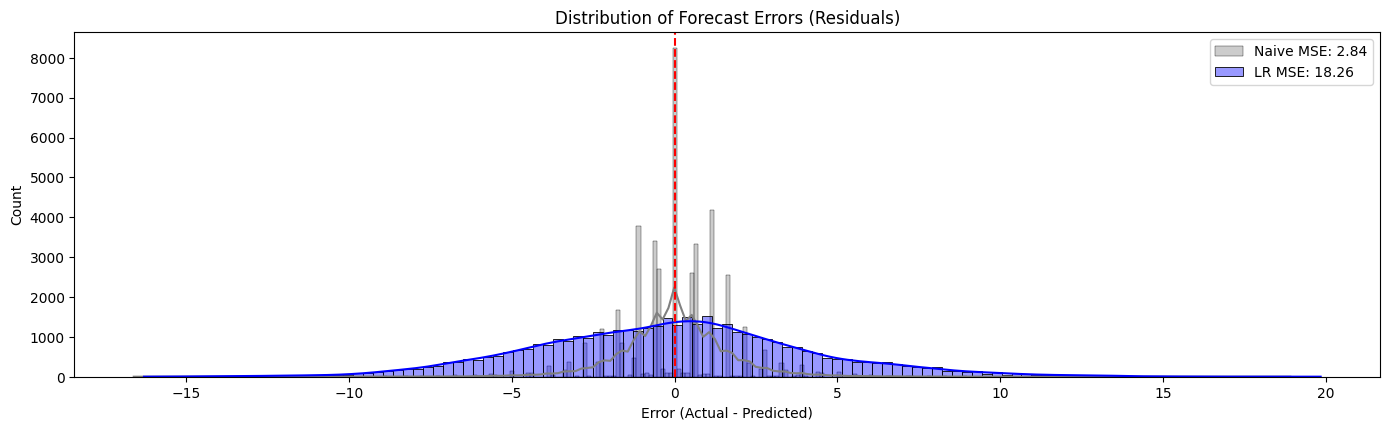
\includegraphics[width=\linewidth]{figures_forecast/residuals.png}
  \caption{Forecast Error Distribution}
  \label{fig:forecast_error_dist}
\end{figure}
\FloatBarrier

From the distribution of the error illustrated in Figure \ref{fig:forecast_error_dist} we can see how the error for the Naive model it's much more centered around the 0 as compared to the Linear Regression Model, which has it error much distributed along line and less predictable of where it can be. This ultimately underscores how the Naive model is a better predictor for short-term intervals because it focuses its prediction based on the current state of the atmosphere rather than trying to fit a general daily trend.

Ultimately, after conducting such preparation before the actual implementation of our SARIMAX model, it became clear that for a forecast model to be successful it must account for both the cyclical nature of time and the high degree of persistence in micro-climate data. These preliminary findings provided the necessary justification to move away from general regression and toward a model that incorporates autoregressive "memory" to handle the short-term dependencies we observed.

\section{Time Series Forecasting}

As the next step, we obviously observed that this data is in a time series format and wanted to use that for the forecasting. For that, we used the \texttt{time\_series\_forecast.ipynb} notebook, where we load the merged dataset, isolate the temperature data, and begin with visualization for the trend, seasonal components, and their residuals. Figure~\ref{fig:hourly} shows the raw hourly series. Even in the first plot, it is easy to notice both the slow seasonal movement from winter to summer and the faster temperature oscillations within each day. Therefore, we intuitively wanted to test monthly and daily seasonal ARIMA forecasting.

\FloatBarrier
\begin{figure}[htbp]
  \centering
  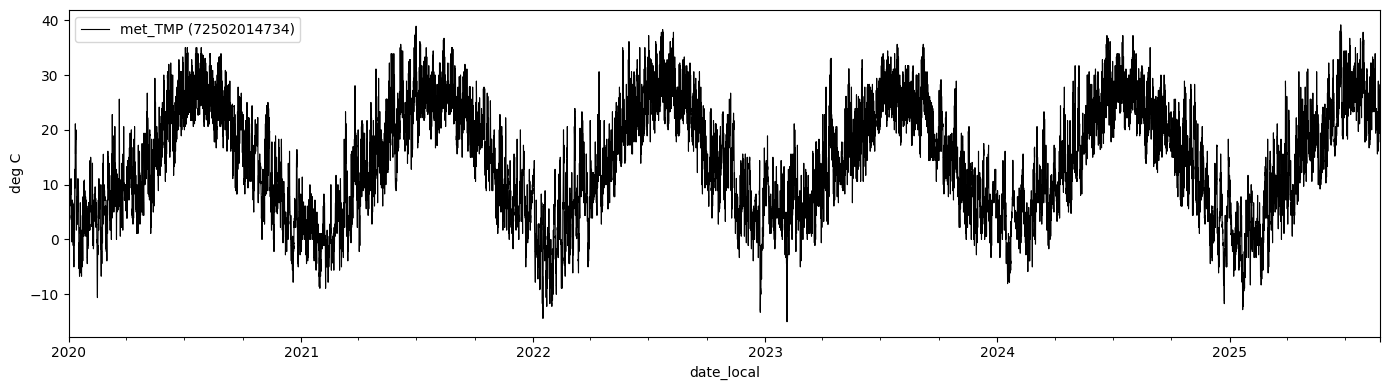
\includegraphics[width=\linewidth]{figures_forecast/hourly_temperature_series.png}
  \caption{Hourly temperature at Newark}
  \label{fig:hourly}
\end{figure}
\FloatBarrier

To better separate those time scales, we plotted rolling means using both 24-hour and 30-day windows. The 24-hour average tracks the daily cycle, while the 30-day average smooths the data into the monthly-basis weather trends, as shown in Figure~\ref{fig:rolling}.

\FloatBarrier
\begin{figure}[htbp]
  \centering
  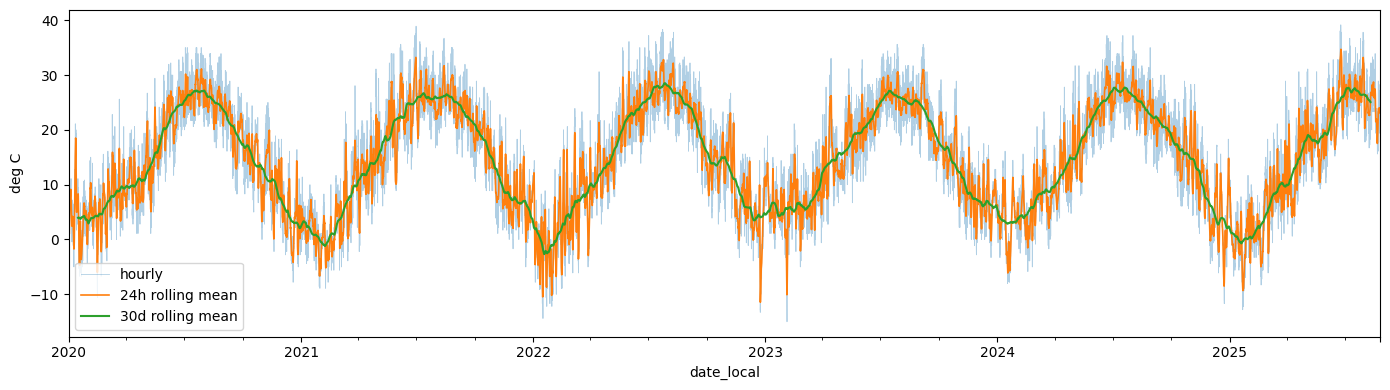
\includegraphics[width=\linewidth]{figures_forecast/rolling_mean_smoothing.png}
  \caption{Rolling averages}
  \label{fig:rolling}
\end{figure}
\FloatBarrier

Next, we applied additive seasonal decomposition with period 24 to the hourly series. In Figure~\ref{fig:stl}, the seasonal component clearly repeats with a recognizable daily structure, while the residual component still contains noticeable variation and spikes. This basically told us that even a seasonal ARIMA-style model is not going to perfectly explain every weather fluctuation. We also examined the autocorrelation and partial autocorrelation plots on a de-meaned subset of the data. Figure~\ref{fig:acf} shows strong spikes at multiples of 24 hours, which reinforced the idea that a seasonal period of $s=24$ would likely be important.

\FloatBarrier
\begin{figure}[htbp]
  \centering
  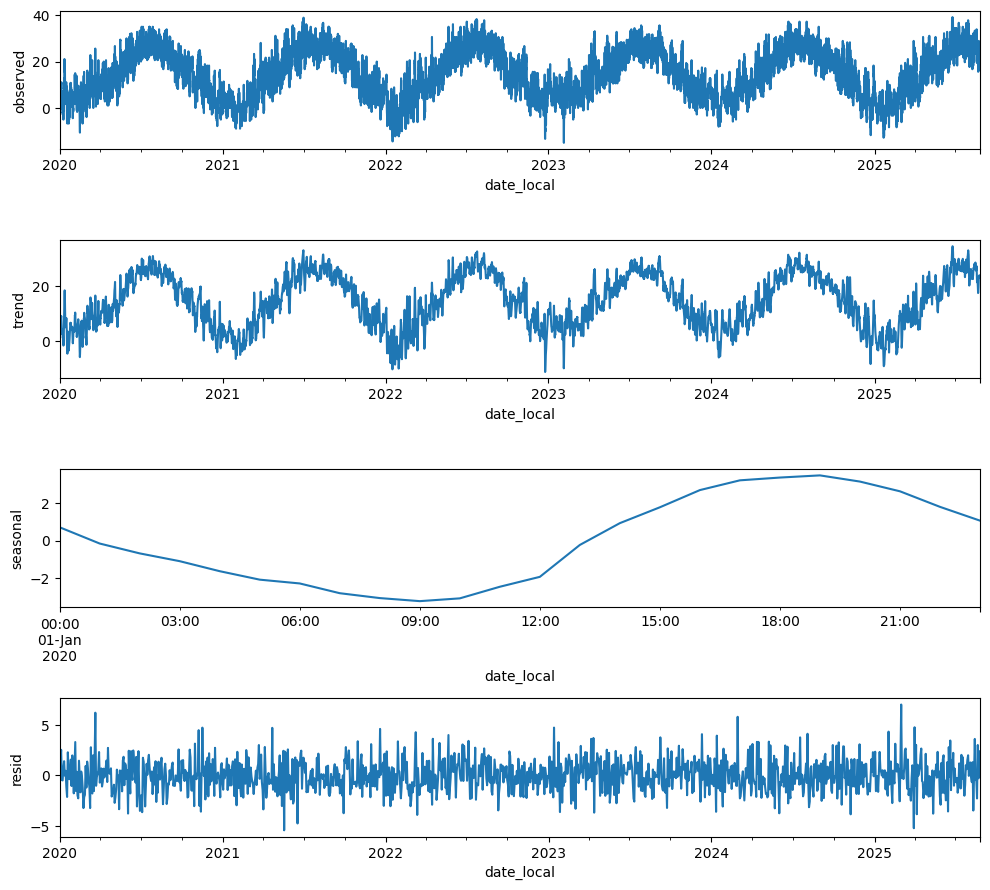
\includegraphics[width=\linewidth]{figures_forecast/seasonal_decomposition.png}
  \caption{Decomposition into trend, daily seasonal component, and residuals}
  \label{fig:stl}
\end{figure}
\FloatBarrier

\begin{figure}[htbp]
  \centering
  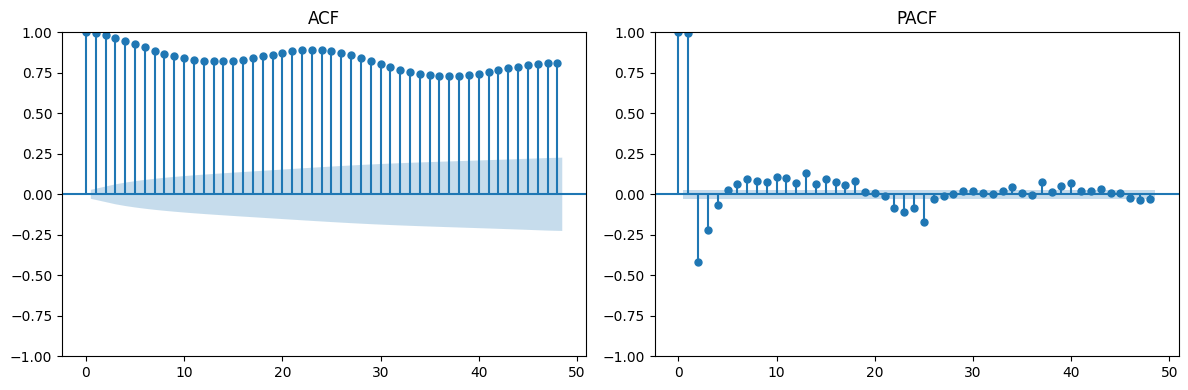
\includegraphics[width=\linewidth]{figures_forecast/acf_pacf.png}
  \caption{ACF/PACF after subtracting the mean on the train data}
  \label{fig:acf}
\end{figure}
\FloatBarrier

Our first forecasting model followed fairly directly from those diagnostics. We fit a SARIMAX model on the hourly training data using non-seasonal orders $(1,1,1)$ (our intuition suggested that having just one autoregressive and one moving average terms would be plenty, as there is less likely to be dependence on previous hours' temperatures) and seasonal orders $(1,0,1,24)$ so that the seasonal period corresponded to one day. The resulting forecasts captured the general day-versus-night oscillation reasonably well, but they struggled whenever the slower weather level shifted over longer periods. On the overlapping 2025 test data, this baseline model produced a mean absolute error around $6.9\,^\circ\mathrm{C}$, shown in Figure~\ref{fig:baseline}.

\FloatBarrier
\begin{figure}[htbp]
  \centering
  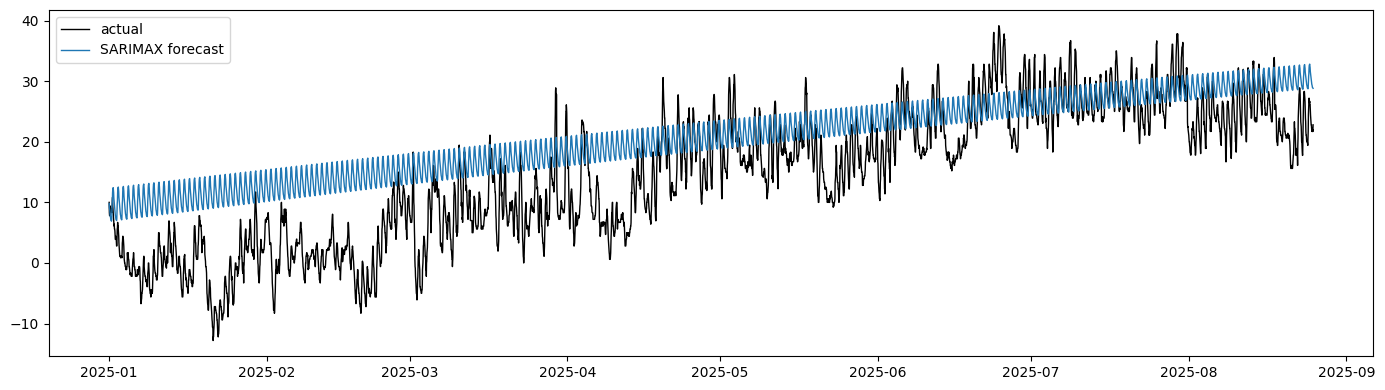
\includegraphics[width=\linewidth]{figures_forecast/sarimax_baseline_forecast.png}
  \caption{Hourly SARIMAX against actual data over test data}
  \label{fig:baseline}
\end{figure}
\FloatBarrier

We then explored whether modeling slower trends separately would help. To do that, we averaged temperatures into monthly values and fit a second SARIMAX model using yearly seasonality with period 12. The monthly forecasts were then broadcast back across every hour within each month (we thought there might be better ways to do this since it's likely that the start of March would be colder than the end of March, but we didn't find any easy way to do that apart from breaking the seasonality into finer monthly components). Interestingly, this monthly-only approach achieved roughly $4.4\,^\circ\mathrm{C}$ MAE on the same test data, outperforming the purely hourly model. That suggested much of the baseline error came from missing the broader temperature level rather than the hourly oscillations themselves.

After that, we experimented with a linear combination of the hourly and monthly forecasts. We swept through several linear combinations to see whether combining the two models would improve performance. Many blended forecasts landed somewhere between the two individual models, although the best-performing versions leaned heavily toward the monthly component (matter of fact, our grid-based search suggested that the best weights were 0.0 for the hourly model and 1.0 for the monthly model). In basically all cases, adding too much of the hourly model actually hurt performance by reintroducing noisy short-term variation. We still implemented the 0.1 x Hourly Forecast + 0.9 x Monthly Forecast model as it was the second best performing linear combination, but it was surprising to see the pure monthly model outperform it. 

\FloatBarrier
\begin{figure}[htbp]
  \centering
  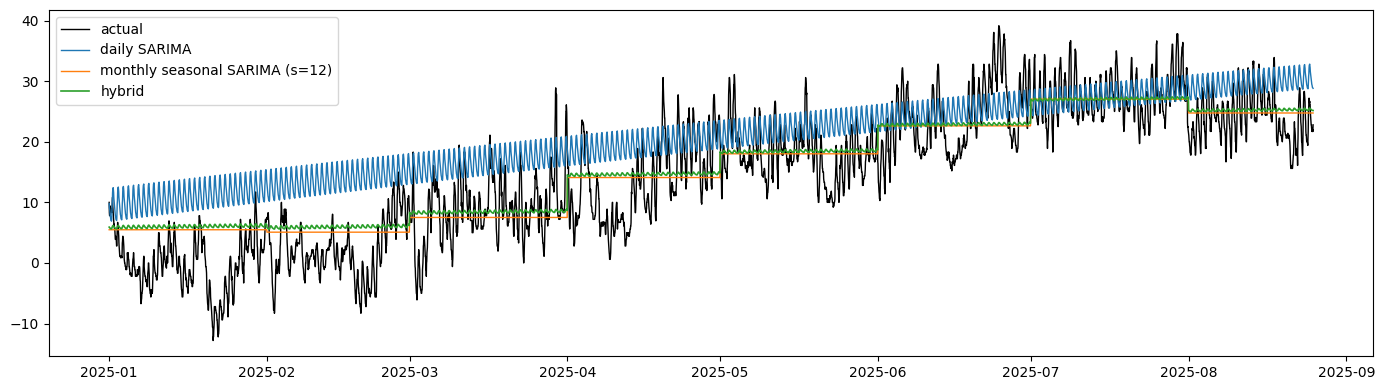
\includegraphics[width=\linewidth]{figures_forecast/hybrid_linear_blend.png}
  \caption{Hourly SARIMAX, monthly SARIMAX, and a 0.1 \& 0.9 combination on the test split}
  \label{fig:hybrid}
\end{figure}
\FloatBarrier

Although the blending approach improved results somewhat, it felt a little improvised. We therefore moved toward a more structured hierarchical method that better matched the patterns we observed earlier in the rolling averages. First, we fit the monthly SARIMAX model again and mapped its fitted monthly level onto each hourly timestamp in the training data. We then subtracted this slow-moving level from the raw hourly temperatures and trained a second SARIMAX model on the residual series using seasonal period 24. In this stage, we removed non-seasonal differencing because the long-term trend had already been handled by the monthly component. During forecasting, we added the monthly forecast back onto the predicted hourly residuals to get the hierarchical forecast.

This hierarchical approach produced forecasts that visually tracked the observed temperature series more closely, as shown in Figure~\ref{fig:hierarchical}. The MAE dropped further to around $4.1\,^\circ\mathrm{C}$, outperforming both the original hourly-only, monthly-only, and the linear combination models. We also found this setup easier to explain conceptually, since the monthly model captures slow seasonal movement while the hourly model focuses only on short-term residual behavior.

\FloatBarrier
\begin{figure}[htbp]
  \centering
  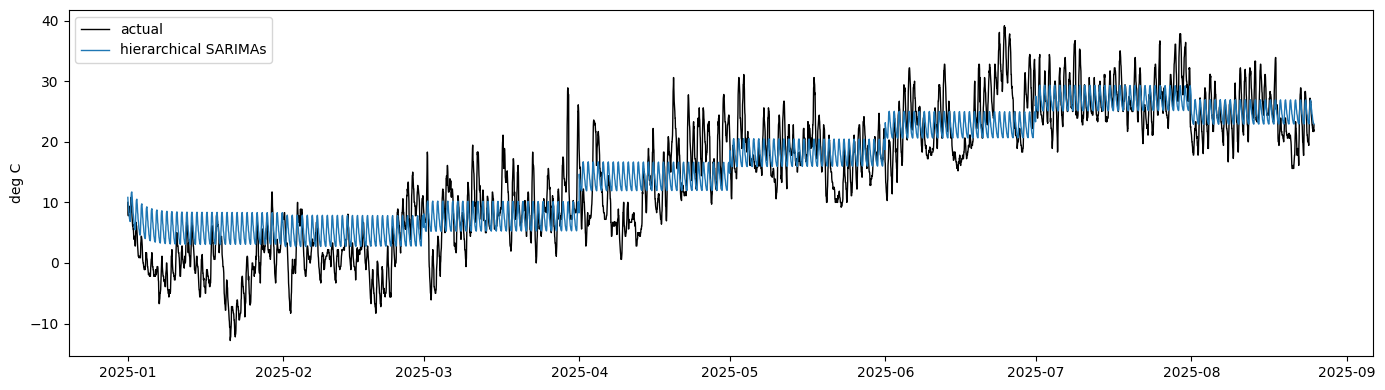
\includegraphics[width=\linewidth]{figures_forecast/hierarchical_forecast.png}
  \caption{Hierarchical SARIMAX}
  \label{fig:hierarchical}
\end{figure}
\FloatBarrier

Overall, even a time-series based approach yielded a 4.1 degree Celsius MAE on the test set, which is a significant improvement over the baseline model but is not perfect by all means since it fails to capture the finer patterns in the data.

\section{Outcomes and Discussion}
To conclude our experimental results for this report, once again the linear regression approach for predicting temperature between short intervals, hourly, is unsatisfactory. While the most simplest Naive approach predicting the next hour's temperature using the current "observed value" does a much better job ($MSE = 2.84$ vs. $18.26$ for Linear Regression). However for long-term forecasting where daily and monthly-seasonal patterns does play a role, the hierarchical SARIMAX model is a reliable method. Unlike the Naive, which relies purely on immediate temporal persistence, the hierarchical SARIMAX captures the physical reality of the atmosphere. By breaking down the data into a monthly seasonal model ($h=24\times30$) and an hourly residual model ($h=24$), we successfully accounted for both slow-moving climate trends and, in comparison, on a faster daily hourly basis. 

Later on the hierarchical approach that was implemented separates the monthly seasonal trend from the hourly residuals which allows the model to overcome the high bias seen in the baseline as explained in the Time Series Forecasting section. The application of $(1, 1, 1) \times (1, 0, 1, 24)$ to the hourly residual enables us to capture the hourly-daily cycle that the monthly model would have missed, and as for incorporate the stability from the monthly-seasonally model into the hourly-model. The hierarchical is an overall winner since it's combined with the advantages of both the daily and monthly SARIMAX model.

Something to note before the end of this report is that even though the Naive MSE (2.84) does looks smaller than our final MAE (4.1), we need to be aware that these are two different units, MAE is measured in actual degrees ($^{\circ}C$), providing a clear, functional error for real-world use, whereas MSE is in degrees squared ($^{\circ}C^2$). Beyond theses different unit of measure, the Naive model’s usefulness basically evaporates the moment when you try to forecast more than a single hour ahead, unlike the SARIMAX approach which handles longer horizons.
    
\section{Limitations}
As mentioned earlier in this report, the testing period extends through $2026-01-01$. However, the Newark dataset only included observations up to August 2025. As a result, the model was unable to evaluate weather behavior during the final months of 2025. This creates an important limitation because the test-set results do not fully capture potential late-year volatility, seasonal fluctuations, or overall year-end performance that could have affected the accuracy of the forecasts.

In addition, neither of the SARIMA models currently used in this project incorporates external variables beyond the hourly and monthly seasonal components. Factors such as rainfall, storms, humidity, or other weather-related events were not included in the forecasting process but are obviously likely to be impactful (e.g. it is likely that a day with rain will have lower temperatures than a sunny day). Instead, the models rely entirely on historical temperature patterns when generating future predictions. While this approach still captures general trends and seasonality, it may reduce forecasting accuracy during unusual or rapidly changing weather conditions, so we would want to tap into the rest of the available data for the future extensions of this project.

Another limitation is that several additional variables available through the NOAA datasets were not included in the final model. Data such as wind speed, wind direction, atmospheric pressure, and related environmental measurements were accessible during the project but ultimately not incorporated into the forecasting logic. The current implementation focuses primarily on temperature data when producing predictions. Including these extra climate variables in future versions of the model could potentially improve performance by allowing the forecasts to account for a broader range of weather dynamics. During this project's implementation, we even contemplated making a simple machine learning model to evaluate the significance of the available factors for the temperature forecasting, which would be another great comparison for the future, and a useful input into the final SARIMA forecast.

\section*{References}

\medskip
{
\small
[1] Shi, X., Chen, Z., Wang, H., Yeung, D.Y., Wong, W.K., \& Woo, W.C. (2015). Convolutional LSTM network: A machine learning approach for precipitation nowcasting. \textit{In Advances in Neural Information Processing Systems}.

[2] NOAA National Centers for Environmental Information. Climate Data Online (CDO). \url{https://www.ncei.noaa.gov/cdo-web/} Accessed: 2026-03-15.

[3] NOAA National Centers for Environmental Information. Local Climatological Data (LCD). \url{https://www.ncei.noaa.gov/products/land-based-station/local-climatological-data}

[4] NOAA National Centers for Environmental Information. Global Hourly - Integrated Surface Database. \url{https://www.ncei.noaa.gov/products/land-based-station/integrated-surface-database}
}

\end{document}